%% Evaluation
%!TEX root = ../Project.tex
\section{Evaluation and Critical Appraisal}

\subsection{Objectives}
\label{sub:eobjectives}
The objectives, as listed in section \ref{sub:objectives},  are extensive, ranging from primary objectives that required a basic engine capable of creating a Tactical RPG to tertiary objectives which required the creation of an editor which customised most aspects of the  engine. 

Since all the primary and secondly objectives were completed, as well as nearly all the tertiary objectives I consider  the project a success, I will now discuss the objectives in details.

\subsubsection{Primary Objectives}

The primary objectives focus on the basic functionality of the engine, I have marked these objectives as completed. Notable improvements from the objectives include the engine handling the pagination and line wrapping of the dialog automatically, which frees the user from fiddling with the dialog to make it fit on the screen. 
% in an astecly pleseing wayN

Combat between units was a primary requirement which was completed with many additional features, which are discussed later.

The primary requirements were to make an isometric graphical representation of the game, this was very successful. The view had useful features such as it allows the game to played with either the mouse or the keyboard.

\subsubsection{Secondary Objectives}
The main goal of the secondary objectives is to allow the user more customisability.  Associating attributes such as height and movement cost to the tiles was a requirement that was completed. In addition, the engine support \emph{empty} tiles which are impassable are not displayed to the user. This allows the creation of more complex maps as shown in figure \ref{fig:figures_editor_Map}. Another enhancement is that \emph{slated} tiles can be used, they are tiles that have a different start and end height and could be used for making stairs or cliffs. 

The secondary objectives required a combat system that supports the use of weapons and non-adjacent targets for both the player and the AI opponent. Weapons in particular deserve  mention since they are completely configurable. The engine, of course, provides default implementations of common weapons such as ranged weapons and spears (which shows the weapons can have extra effects such as attacking multiple targets). 

The default implementation  of the battle (The user can use their own battle system, but it is more complex) takes many attributes such as the units' levels and difference in height between the attack and the target to determine the outcome of a battle. 

I completed the objective of allowing music and sound effects, the format used is Ogg Vorbis (Appendix \ref{sub:music}). In addition, wave files can be used for sound effects, this was implemented since the format seems to be commonly used for this purpose.

Saving and loading the game were implemented as required, but with the restriction that when a save file is loaded, the player begins at the \emph{beginning} of the last played map.

Allowing the user to customise the AI behaviour is a completed objective. In addition, the engine provides default behaviours including the example of attacking the player's unit with the lowest HP. The engine also provides default actions such as while moving to a faraway target if the target is not reachable, move as close as possible and attack any opposing player's units that are in reach. 

\subsubsection{Tertiary Objectives}
The main objectives of these requirements was to produce an editor that allowed customising of most aspects of the engine as well as combat improvements and units animations, all of them having been completed. 

Combat requirement improvements include \texttt{skills} that can affect multiple units, and weapons which can attack multiple units. Further enhancements to this system include complete customisable range (e.g could be used to attack all enemy units around the attack).

The requirement for animated unit movement was completed. This was further improved by taking account of the direction the unit is traveling in, which was done by having an  image for each of the four directions. 

\paragraph{Editor\\}
An editor that can customise nearly all aspects of the engine was created.  The most prominent features are the visual map editor (section ref), unit creation(section ref), dialog editing(section ref) and exporting as a self contained application.  The editor met all the  tertiary requirements and it also had addition improvements. These include an easy to edit dialog format for importing/exporting and inter-compatibility  with Stasyk’s Terrain Generator to give a user a start point for their map designs.

%TODO more? section refs

\paragraph{Scripting \& Custom Events\\}
A tertiary requirement was to implement custom events through the use of scripting.  This would allow the user to specify events such as making the player win if some enemies unit has less then 50\% Hit Points. 

To implement this I had planned to use the Java Scripting API\cite{javas}. The would allow embedding a dynamic scripting language.  The main benefit of this is that the code does not have to be compiled, which means it does not have the same hurdles with class linking as my Extension Mechanism(Appendix \ref{sub:data_format_extension_mechanism}).   The language chosen for embedding was Javascript  as it is built into the JDK, so the user does not have to install anything extra and of all the scripting languages, Javascript  is more likely to have been used before by the average user, these decisions are described in more detail in appendix \ref{sec:Scripting}. 

Some people such as ref  advocate forgoing scripting completing, pointing out that scripting is a lazy of letting users have customisability since it can be quite difficult for users to create events.  Using their advice of creating visual editors for creating events and customising unit behaviours, I allowed the user to specify common events from the editor, with the option of linking they own classes as a last resort. 

Although the scripting was not implemented due to time constraints, note that it was a tertiary objective and all the given examples in the objective are supported by the engine. In particular, win conditions can be specified (section ref) and common winning conditions can even can be selected from the editor.  The engine supports showing dialog at arbitrary points in the game which could be used to support the requirement ``Showing some part of the story when a player’s character reaches a specified tile''.

The engine supports the user using their own classes through the extension mechanism in Appendix \ref{sub:data_format_extension_mechanism}, which allows a slightly more limited form of scripting but with the benefit of being type safe and with the drawback of being more complex.
% ref game progamming gems

% morrowind 
% wow 
% never winter nights 
% 

\subsection{Comparison to Similar Work}
\subsubsection{Engine}
\label{ssub:engine}

The capabilities of the engine will be compared and contrasted with the games discussed in the context survey(section \ref{Context_Survey}).  Like most of the games described before, the engine supports an isometric view point which allows the user to create aesthetically pleasing map.  
	
In particular, the turning ordering is very general to the extent that the user can completely replace it with their own code, all the described game ordering systems could be implemented.  The default system resembles the ordering used in \texttt{Tactics Ogre}, as a example the supported features. 

Nearly all TRPGs  include weapons and  skills (sometimes having other names such as `magic'). The engine fully supports this, and even has additional features such as arbitrary ranges (This is where the attack range of a weapon or skill can be in any shape and size. The weapon type \texttt{around}, which attacks all enemies in all the tiles around the attacker, was created as an example of this.)

Like practically all TRPG, the engine has a battle system with support for weapons, skill and which takes account of the terrain of the map.  The main features the engine is missing is \emph{uncertainty} that actions have a small chance of missing, or have an unintended consequence. This quite common feature, an example is attack missing or bow hitting an allied unit that was in the way. At the moment the engine carries out all of the users requested actions without fail, which is in some ways better since it is more predictable, hence making it easier.  

Although the engine supports units levelling up and having the attributes increased, it does not support restricting  skills to a specific level, that is a unit knows all of it's skills at the beginning. In contrast, most TRPG usually restrict a unit's skills to a select few at the beginning, the unit then gains new skills as it levels up. This was not an of the objective of the project, but will be considered for future work.

The main feature that is lacking from the engine is an overworld map. An overworld map has a series of user selectable locations, where the battles take place in each location, this is common in nearly all TRPG (although is deliberately omitted from the discussed ``Fire Emblem'' series). This was not an objective of the project because it would time consuming to make the overworld maps. Nevertheless, I tried to implement this, the overworld maps are quite smiler to  Sasha generated maps, by giving him the idea for place names (randomly generated) at suitable locations.  He was able to generate overworld maps that I could use. Due to time constraints this was not implemented, but will probably be carried out as future work. For an example of what it would look like see (section ref)

\subsubsection{Editor}
\label{ssub:editor}
Since \texttt{Simulation Maker 95}(SM) is one of the only completed Tactical RPG creators, it will be used for evaluating the Editor.  Both editors support visual map editing but differ in the type of map created,  my editor supports the now more common isometric viewpoint where as SM only supports a topdown view. 

Whereas SM only allows changing the win conditions, my editor allows customising most aspects of the engine, including the win conditions and enemy behaviour.  Another advantage my editor has over SM is image loading, my editor provides a visual interface that allows the user to import images in any of the Java supported image formats(which include, jpeg, gif and png) whereas in SM the user has to place the images in the right directory with the correct names, furthermore it only supports bitmaps, meaning that any significant uses of images would lead to huge file sizes.  

One of the major features that is not present in SM is the ability to export a cross-platform jar that will work on any Java enabled platform, this is in contrast to SM which only works in windows, and can only export games for windows.


% ref example reportt
\subsection{Results of User Testing}
\label{sub:results_of_user_testing}

In total six participants took part in the user testing, more people were interested but could not due to time constraints.  See Appendix \ref{sec:questionnaire} for the Questionnaire.

\subsection{Analysis of User Responses}
The participants can be grouped into three groups, those who have played a TRPG before, those who have not and those who don't play games at all.
\paragraph{Feedback from  all groups\\}
Both groups thought the editor supported all the features they would like if they created a TRPG.  Most of the participants answered that they would like to use the editor again.  Interestingly, all users who were familiar with TRPG used the keyboard exclusively, this I attribute to participants being used to the input mechanism since most TRPG are on consoles\footnote{such as Playstation 2}. Those who had no experience playing TRPG unexpectedly used both the keyboard and mouse at the same time (generally selecting the units with the mouse then using the keyboard for performing any actions).

\paragraph{Feedback from those who had played a TRPG before\\}
Participants that had experience playing a TRPG before found the engine very intuitive. They especially liked how everything was customisable.  The visual map editor also gained significant praise for it's easy of use and it's range of features.  Other features that participants liked were how a project could be exported as a standalone Mac OS X application with virtually no effort. 

When playing the pre-created game, all of the participants were able to play, and even win, the game!. Some of the participants were able to figure out all of the out the controls with out even reading the help screen. 

\paragraph{Feedback from those who had not played a TRPG  before\\} 
In contrast, participants who never played a TRPG before felt overwhelmed with the available options, although they figured how to use it quite quickly.  They particularly liked how robust the editor was. The main features that were requested were  an overview of each feature in the editor and how they interacted.  The participants commented on the pleasing visual appearance of the editor.

When playing the pre-created game, some of the participants were initially confused by the interface. All participant were able to finish the game even if they could not win.  The participant unexpectedly kept on using the enter key to perform actions on the unit even though the help panel stated otherwise. In response to this feedback, I added the enter key as an alias of the action key(default `x').

\subsubsection{System Usability}
A System Usability Scale (SUS) was used \cite{SUS}. This works by giving each even numbered questions a score of (5 - \emph{value}) and odd numbered questions a score of (\emph{value}-1). Questions that contributed to a high score showed that the system is usable. 

Based on this schema, the maximum positive contribution is four. To get the overall usability score, the sum of the questions contributions is multiplied by 2.5.  This gives  a score out out of 100, which is easier to understand and use for statistical purposes.

\paragraph{Results\\}
Since the average scores(figure \ref{fig:figures_SUS_Mean}) were at lest two (the middle value), which means that users responses tended to be positive. 

\paragraph{Analysis\\}

The system performed well in user testing, receiving a usability score of 62.4, out of 100. Taking into account that many of the users had never played a Tactical RPG before this is definitely a positive score. 

The usability result was 61. This is a very good result since a score of 50 means that the system is useable. Although there is room for improvement, the usability testing shows the system has achieved the goal of being useable.

\begin{figure}[htb]
	\centering
		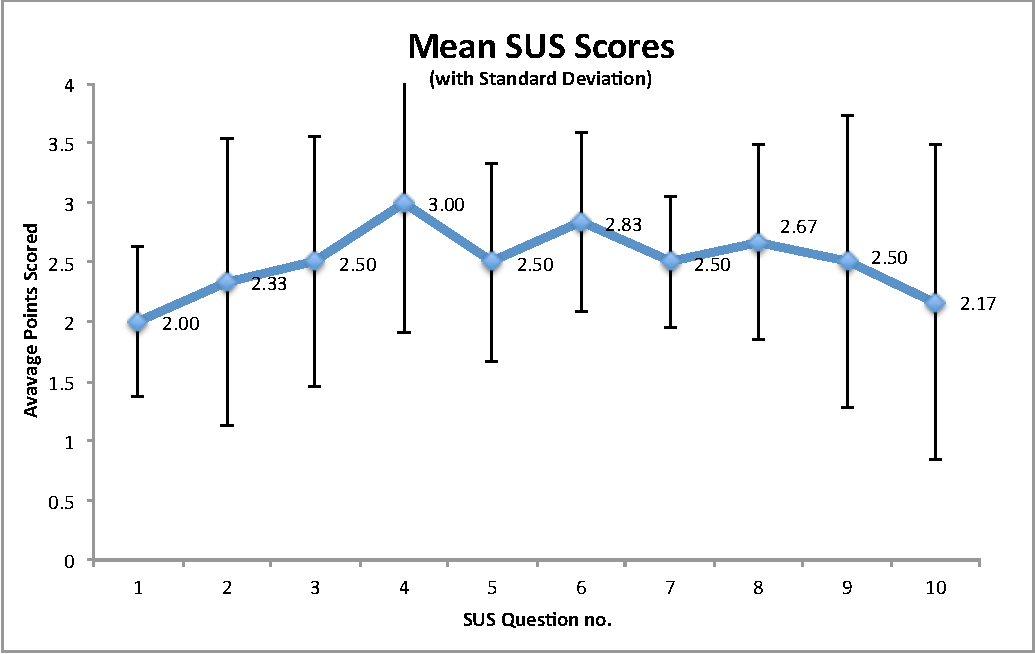
\includegraphics[height=3in]{figures/SUS_Mean.pdf}
	\caption{Mean System Usability Contributing Scores, the user responses were generally positive.}
	\label{fig:figures_SUS_Mean}
\end{figure}

\begin{figure}[htb]
	\centering
		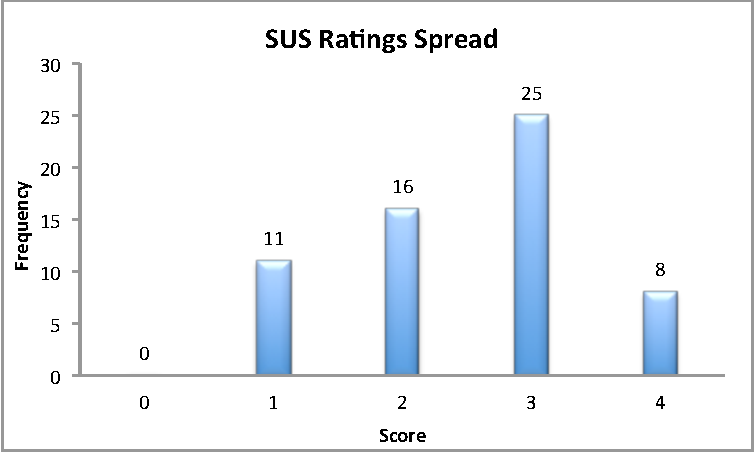
\includegraphics[height=3in]{figures/SUS_Spread.pdf}
	\caption{Spread of the user's scores.}
	\label{fig:figures_SUS_Spread}
\end{figure}